
%%%%%%%%%%%%%%%%%%%%%%%%%%%%%%%%%%%%%%%%%%%%%%%%%%%%%%%%%%%%%%%%%%%%%%%%%%%%%
\chapt[chap:annic]{ANNIC: ANNotations-In-Context}
\markboth{ANNIC: ANNotations-In-Context}{ANNIC: ANNotations-In-Context}
%%%%%%%%%%%%%%%%%%%%%%%%%%%%%%%%%%%%%%%%%%%%%%%%%%%%%%%%%%%%%%%%%%%%%%%%%%%%%
\nnormalsize

%%%%%%%%%%%%%%%%%%%%%%%%%%%%%%%%%%%%%%%
%\sect[sec:misc-creole:annic]{ANNIC}
ANNIC (ANNotations-In-Context) is a full-featured annotation indexing and 
retrieval system.  It is provided as part of an extension of the Serial 
Data-stores, called Searchable Serial Data-store (SSD).

ANNIC can index documents in any format supported by the GATE system
(i.e., XML, HTML, RTF, e-mail, text, etc). Compared with other such query
systems, it has additional features addressing issues such as extensive indexing 
of linguistic information associated with document content, independent of 
document format. It also allows indexing and extraction of information from 
overlapping annotations and features. Its advanced graphical user interface 
provides a graphical view of annotation markups over the text, along with an 
ability to build new queries interactively. In addition, ANNIC can be used as 
a first step in rule development for NLP systems as it enables the discovery 
and testing of patterns in corpora. 

ANNIC is built on top of the Apache
Lucene\footnote{http://lucene.apache.org} -- a high performance full-featured
search engine implemented in Java, which supports indexing and search of large
document collections. Our choice of IR engine is due to the customisability of
Lucene. For more details on how Lucene was modified to meet the requirements of
indexing and querying annotations, please refer to \cite{Aswani05}.

As explained earlier, SSD is an extension of the serial data-store. In
addition to the persist location, SSD asks user to provide some more
information (explained later) that it uses to index the
documents. Once the SSD has been initiated, user can add/remove
documents/corpora to the SSD in a similar way it is done with other
data-stores.  When documents are added to the SSD, it automatically
tries to index them. It updates the index whenever there is a change
in any of the documents stored in the SSD and removes the document
from the index if it is deleted from the SSD. Be warned that only the
annotation sets, types and features initially provided during the SSD creation 
time, will be updated when adding/removing documents to the datastore.

SSD has an advanced graphical interface that allows users to issue
queries over the SSD.  Below we explain the parameters required by SSD
and how to instantiate it, how to use its graphical interface and how
to use SSD programmatically.

%%%%%%%%%%%%%%%%%%%%%%%%%%%%%%%%%%%%%%%%%%%%%%%%%%%%%%%%%%%%%%%%%%%%%%%%%%%%%
\sect[sec:annic:instantiating-ssd]{Instantiating SSD}
%%%%%%%%%%%%%%%%%%%%%%%%%%%%%%%%%%%%%%%%%%%%%%%%%%%%%%%%%%%%%%%%%%%%%%%%%%%%%

Steps:
\begin{enumerate}
\item In GATE Developer, right click on `Datastores' and select `Create Datastore'.
\item From a drop-down list select `Lucene Based Searchable DataStore'.
\item Here, you will see a file dialog. Please select an empty folder for your
datastore. This is similar to the procedure of creating a serial datastore.
\item After this, you will see an input window. Please provide these parameters:
\begin{enumerate}
\item DataStore URL:  This is the URL of the datastore folder selected in the 
previous step.
\item Index Location:  By default, the location of index is calculated from the 
datastore location. It is done by appending `-index' to the datastore location.
If user wants to change this location, it is possible to do so by clicking on 
the folder icon and selecting another empty folder.  If the selected folder
exists already, the system will check if it is an empty folder. If the selected 
folder does not exist, the system tries to create it.
\item Annotation Sets:  Here, you can provide one or more annotation sets that
you wish to index or exclude from being indexed. By default, the default 
annotation set and the `Key' annotation set are included.  User can change this 
selection by clicking on the edit list icon and removing or adding appropriate 
annotation set names.  In order to be able to readd the default annotation set, 
you must click on the edit list icon and add an empty field to the list. If 
there are no annotation sets provided, all the annotation sets in all documents 
are indexed.
\item Base-Token Type:  (e.g. Token or Key.Token)  These are the basic tokens of
any document.  Your documents must have the annotations of
Base-Token-Type in order to get indexed.  These basic tokens are used for
displaying contextual information while searching patterns in the corpus.
In case of indexing more than one annotation set, user can specify the
annotation set from which the tokens should be taken (e.g. Key.Token- 
annotations of type Token from the annotation set called Key).  In case user 
does not provide any annotation set name (e.g. Token), the system searches in 
all the annotation sets to be indexed and the base-tokens from the first 
annotation set with the base token annotations are taken. Please note that the 
documents with no base-tokens are not indexed. However, if the `create tokens 
automatically' option is selected, the SSD creates base-tokens automatically. 
Here, each string delimited with white space is considered as a token.
\item Index Unit Type: (e.g. Sentence, Key.Sentence) This specifies the unit of 
Index. In other words, annotations lying within the boundaries of these 
annotations are indexed (e.g. in the case of `Sentences', no annotations that
are spanned across the boundaries of two sentences are considered for indexing).
User can specify from which annotation set the index unit annotations should be
considered.  If user does not provide any annotation set, the SSD searches among
all annotation sets for index units. If this field is left empty or SSD fails to
locate index units, the entire document is considered as a single unit.
\item Features:  Finally, users can specify the annotation types and features 
that should be indexed or excluded from being indexed. (e.g. SpaceToken and 
Split). If user wants to exclude only a specific feature of a specific 
annotation type, he/she can specify it using a '.' separator between the 
annotation type and its feature (e.g. Person.matches).
\end{enumerate}
\item Click OK.  If all parameters are OK, a new empty DS will be created.
\item Create an empty corpus and save it to the SSD.
\item Populate it with some documents. Each document added to the corpus and
eventually to the SSD is indexed automatically. If the document does not have
the required annotations, that document is skipped and not indexed.
\end{enumerate}

SSDs are portable and can be moved across different systems. However, the 
relative positions of both the datastore folder and the respective index folder
must be maintained. If it is not possible to maintain the relative positions,
the new location of the index must be specified inside the 
`\_\_GATE\_SerialDataStore\_\_' file inside the datastore folder.

%%%%%%%%%%%%%%%%%%%%%%%%%%%%%%%%%%%%%%%%%%%%%%%%%%%%%%%%%%%%%%%%%%%%%%%%%%%%%
\sect[sec:annic:search-gui]{Search GUI}
%%%%%%%%%%%%%%%%%%%%%%%%%%%%%%%%%%%%%%%%%%%%%%%%%%%%%%%%%%%%%%%%%%%%%%%%%%%%%

\begin{figure}
\begin{center}
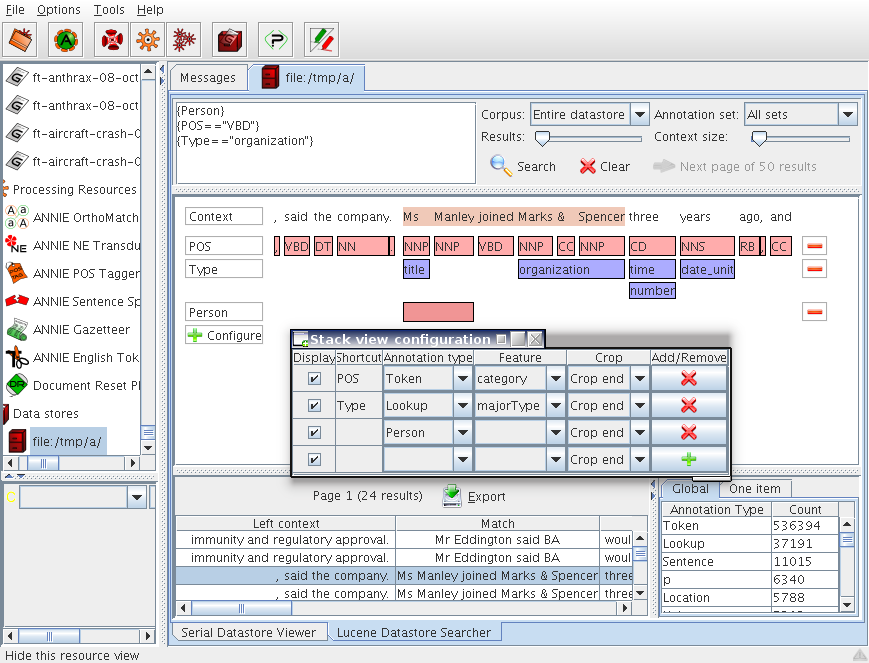
\includegraphics[height=8cm]{ssd.png}
\caption{Searchable Serial Datastore Viewer.}
\label{fig:annicmain}
\end{center}
\end{figure}

\subsect{Overview}

Figure \ref{fig:annicmain} shows the search GUI for a datastore. The top
section contains a text area to write a query, lists to select the corpus
and annotation set to search in, sliders to set the size of the results and
context and icons to execute and clear the query.

The central section shows a graphical visualisation of stacked annotations
and feature values for the result row selected in the bottom results
table. There is a configuration window where you define which annotation
type and feature to display in the central section.

The bottom section contains the results table of the query, i.e. the text
that matches the query with their left and right contexts. The bottom
section contains also a tabbed pane of statistics.

%%%%%%%%%%%%%%%%%%%%%%%%%%%%%%%%%%%%%%%%%%%%%%%%%%%%%%%%%%%%%%%%%%%%%%%%%%%%%
\subsect[sec:annic:query-syntax]{Syntax of Queries}
%%%%%%%%%%%%%%%%%%%%%%%%%%%%%%%%%%%%%%%%%%%%%%%%%%%%%%%%%%%%%%%%%%%%%%%%%%%%%

SSD enables you to formulate versatile queries using a subset of JAPE
patterns. Below, we give the JAPE pattern clauses which can be used as SSD
queries. Queries can also be a combination of one or more of the following
pattern clauses.

\begin{enumerate}
\item String
\item \{AnnotationType\}
\item \{AnnotationType == String\}
\item \{AnnotationType.feature == feature value\}
\item \{AnnotationType1, AnnotationType2.feature == featureValue\}
\item \{AnnotationType1.feature == featureValue, AnnotationType2.feature == featureValue\}
\end{enumerate}

JAPE patterns also support the $|$ (OR) operator. For instance, \{A\} (\{B\} $|$
\{C\}) is a pattern of two annotations where the first is an annotation of type A
followed by the annotation of type either B or C.

ANNIC supports two operators,
+ and *, to specify the number of times a particular annotation or a sub pattern
should appear in the main query pattern. Here, (\{A\})+n means one and up to n
occurrences of annotation \{A\} and (\{A\})*n means zero or up to n occurrences of
annotation \{A\}.

Below we explain the steps to search in SSD.

\begin{enumerate}
\item Double click on SSD. You will see an extra tab ``Lucene DataStore
Searcher''. Click on it to activate the searcher GUI.
\item Here you can specify a query to search in your SSD. The query here is a
L.H.S. part of the JAPE grammar. Here are some examples:

\begin{enumerate}
\item \{Person\}  -- This will return annotations of type Person from the SSD
\item \{Token.string == ``Microsoft''\}  -- This will return all occurrences of
``Microsoft'' from the SSD.
\item \{Person\}(\{Token\})*2\{Organization\} -- Person followed by zero or
up to two
tokens followed by Organization.
\item \{Token.orth==``upperInitial'',  Organization\} -- Token with feature orth
with value set to ``upperInitial'' and which is also annotated as Organization.
\end{enumerate}
\end{enumerate}

\begin{figure}
\begin{center}
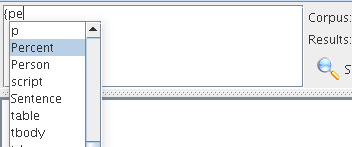
\includegraphics[height=4cm]{ssd-auto-completion.png}
\caption{Searchable Serial Datastore Viewer - Auto-completion.}
\label{fig:annic-auto-completion}
\end{center}
\end{figure}

%%%%%%%%%%%%%%%%%%%%%%%%%%%%%%%%%%%%%%%%%%%%%%%%%%%%%%%%%%%%%%%%%%%%%%%%%%%%%
\subsect[sec:annic:top]{Top Section}
%%%%%%%%%%%%%%%%%%%%%%%%%%%%%%%%%%%%%%%%%%%%%%%%%%%%%%%%%%%%%%%%%%%%%%%%%%%%%

A text-area located in the top left part of the GUI is used to input a
query. You can copy/cut/paste with Control+C/X/V, undo/redo your
changes with Control+Z/Y as usual. To add a new line, use
Control+Enter key combination.

Auto-completion as shown in figure \ref{fig:annic-auto-completion}
for annotation type is triggered when typing '\{' or ',' and for feature when
typing '.' after a valid annotation type. It shows only the annotation
types and features related to the selected corpus and annotation
set.

If you right-click on an expression it will automatically select the
shortest valid enclosing brace and if you click on a selection it will
propose you to add quantifiers for allowing the expression to appear zero,
one or more times.

To execute the query, click on the magnifying glass icon, use Enter key or
Alt+Enter key combination. To clear the query, click on the red X icon or
use Alt+Backspace key combination.

It is possible to have more than one corpus, each containing a
different set of documents, stored in a single data-store. ANNIC, by
providing a drop down box with a list of stored corpora, also allows
searching within a specific corpus. Similarly a document
can have more than one annotation set indexed and therefore ANNIC also
provides a drop down box with a list of indexed annotation sets for
the selected corpus.

A large corpus can have many hits for a given query. This may take a long
time to refresh the GUI and may create inconvenience while browsing through
results. Therefore you can specify the number of results to retrieve. Use
the {\em Next Page of Results} button to iterate through results. Due to
technical complexities, it is not possible to visit a previous page. To
retrieve all the results at the same time, push the results slider to the
right end.

%%%%%%%%%%%%%%%%%%%%%%%%%%%%%%%%%%%%%%%%%%%%%%%%%%%%%%%%%%%%%%%%%%%%%%%%%%%%%
\subsect[sec:annic:central]{Central Section}
%%%%%%%%%%%%%%%%%%%%%%%%%%%%%%%%%%%%%%%%%%%%%%%%%%%%%%%%%%%%%%%%%%%%%%%%%%%%%

Annotation types and features to show can be configured from the stack view
configuration window by clicking on the {\em Configure} button at the bottom
of the annotation stack. You can also change the feature value displayed by
double clicking on the annotation type name in the first column.

The central section shows coloured rectangles exactly below the spans of
text where these annotations occur. If only an annotation type is displayed,
the rectangle remains empty. When you hover the mouse over the rectangle, it
shows all their features and values in a tooltip. If an annotation type and
a feature are displayed, the value of that feature is shown in the
rectangle.

Shortcuts are expressions that stand for an "AnnotationType.Feature"
expression. For example, on the figure \ref{fig:annicmain}, the
shortcut "POS" stands for the expression "Token.category".

When you double click on an annotation rectangle, the respective query
expression is placed at the caret position in the query text area. If you
have selected anything in the query text area, it gets replaced. You can
also double click on a word on the first line to add it to the query.

%%%%%%%%%%%%%%%%%%%%%%%%%%%%%%%%%%%%%%%%%%%%%%%%%%%%%%%%%%%%%%%%%%%%%%%%%%%%%
\subsect[sec:annic:bottom]{Bottom Section}
%%%%%%%%%%%%%%%%%%%%%%%%%%%%%%%%%%%%%%%%%%%%%%%%%%%%%%%%%%%%%%%%%%%%%%%%%%%%%

The table of results contains the text matched by the query, the contexts,
the features displayed in the central view but only for the matching part,
the effective query, the document and annotation set names. You can sort a
table column by clicking on its header.

You can remove a result from the results table or open the document
containing it by right-clicking on a result in the results table.

ANNIC provides an {\em Export} button to export results into an HTML
file. You can also select then copy/paste the table in your word processor
or spreadsheet.

A statistics tabbed pane is displayed at the bottom right. There is always a
global statistics pane that lists the count of the occurrences of all
annotation types for the selected corpus and annotation set. Double clicking
on a row adds the annotation type to the query.

Statistics can be obtained for matched spans of the query in the results,
with or without contexts, just by annotation type, an annotation type +
feature or an annotation type + feature + value. A second pane contains the
one item statistics that you can add by right-clicking on a non empty
annotation rectangle or on the first column of a row in the central
section. You can sort a table column by clicking on its header.

%%%%%%%%%%%%%%%%%%%%%%%%%%%%%%%%%%%%%%%%%%%%%%%%%%%%%%%%%%%%%%%%%%%%%%%%%%%%%
\sect[sec:annic:ssd-embedded]{Using SSD from GATE Embedded}
%%%%%%%%%%%%%%%%%%%%%%%%%%%%%%%%%%%%%%%%%%%%%%%%%%%%%%%%%%%%%%%%%%%%%%%%%%%%%

\subsect{How to instantiate a searchabledatastore}

\begin{lstlisting}

// create an instance of datastore
LuceneDataStoreImpl ds = (LuceneDataStoreImpl) 
	Factory.createDataStore(``gate.persist.LuceneDataStoreImpl'',
	        dsLocation);

// we need to set Indexer
Indexer indexer = new LuceneIndexer(new URL(indexLocation));

// set the parameters
Map parameters = new HashMap();

// specify the index url
parameters.put(Constants.INDEX_LOCATION_URL, new URL(indexLocation));

// specify the base token type
// and specify that the tokens should be created automatically
// if not found in the document
parameters.put(Constants.BASE_TOKEN_ANNOTATION_TYPE, ``Token'');
parameters.put(Constants.CREATE_TOKENS_AUTOMATICALLY, 
               new Boolean(true));

// specify the index unit type
parameters.put(Constants.INDEX_UNIT_ANNOTATION_TYPE, ``Sentence'');

// specifying the annotation sets "Key" and "Default Annotation Set"
// to be indexed
List<String> setsToInclude = new ArrayList<String>();
setsToInclude.add("Key");
setsToInclude.add("<null>");
parameters.put(Constants.ANNOTATION_SETS_NAMES_TO_INCLUDE, 
                setsToInclude);
parameters.put(Constants.ANNOTATION_SETS_NAMES_TO_EXCLUDE,
	        new ArrayList<String>());

// all features should be indexed
parameters.put(Constants.FEATURES_TO_INCLUDE, new ArrayList<String>());
parameters.put(Constants.FEATURES_TO_EXCLUDE, new ArrayList<String>());

// set the indexer
ds.setIndexer(indexer, parameters);

// set the searcher
ds.setSearcher(new LuceneSearcher());

\end{lstlisting}

\subsect{How to search in this datastore}

\begin{lstlisting}

// obtain the searcher instance
Searcher searcher = ds.getSearcher();
Map parameters  = new HashMap();

// obtain the url of index
String indexLocation = 
	new File(((URL) ds.getIndexer().getParameters()
	.get(Constants.INDEX_LOCATION_URL)).getFile()).getAbsolutePath();
ArrayList indexLocations = new ArrayList();
indexLocations.add(indexLocation);


// corpus2SearchIn = mention corpus name that was indexed here.

// the annotation set to search in
String annotationSet2SearchIn = "Key";

// set the parameter
parameters.put(Constants.INDEX_LOCATIONS,indexLocations);
parameters.put(Constants.CORPUS_ID, corpus2SearchIn);
parameters.put(Constants.ANNOTATION_SET_ID, annotationSet);
parameters.put(Constants.CONTEXT_WINDOW, contextWindow);
parameters.put(Constants.NO_OF_PATTERNS, noOfPatterns);

// search
String query = "{Person}";
Hit[] hits = searcher.search(query, parameters);

\end{lstlisting}
